\chapter{Modèle Solid-On-Solid}

La discrétisation du champ $\phi(\mx,t)$ afin de faire des simulations numériques mène naturellement vers le modèle sur réseau par excellence, le modèle d'Ising. À partir de deux dimensions, ce modèle de particules à interaction avec les plus proches voisins, possède une transition de second ordre depuis une phase ordonnée vers une phase désordonnée. Si lon suppose l'énergie d'interaction entre toutes les particules plus proches voisins égale à $J$, la température critique est $\beta_{C,2D} =  \frac{\ln(1+\sqrt{2})}{2} J \simeq 0.44 J$ en deux dimensions \cite{onsager_crystal_1944}. et $\beta_{C,3D} \simeq 0.22 J$ en trois dimensions \cite{talapov_magnetization_1996} (via des simulations de Monte Carlo).

À basse température $T \less T_C$, le système tend à créer des domaines de magnétisation moyenne opposées induisant des interfaces. Nous rappelons dans ce chapitre quelques notions essentielles sur le modèle d'Ising, sur la manière d'étudier les interfaces dans ce modèle, et une approximation à très basse température qui ne retient que l'information sur l'interface : le modèle Solid-On-Solid.

%%%%%%%%%%%%%%%%%%%%%%%%%%%%%%%%%%%%%%%%%%%%%
    \section{Le modèle d'Ising}
%%%%%%%%%%%%%%%%%%%%%%%%%%%%%%%%%%%%%%%%%%%%%  
\begin{figure}
	\begin{minipage}[t]{0.5\linewidth}
		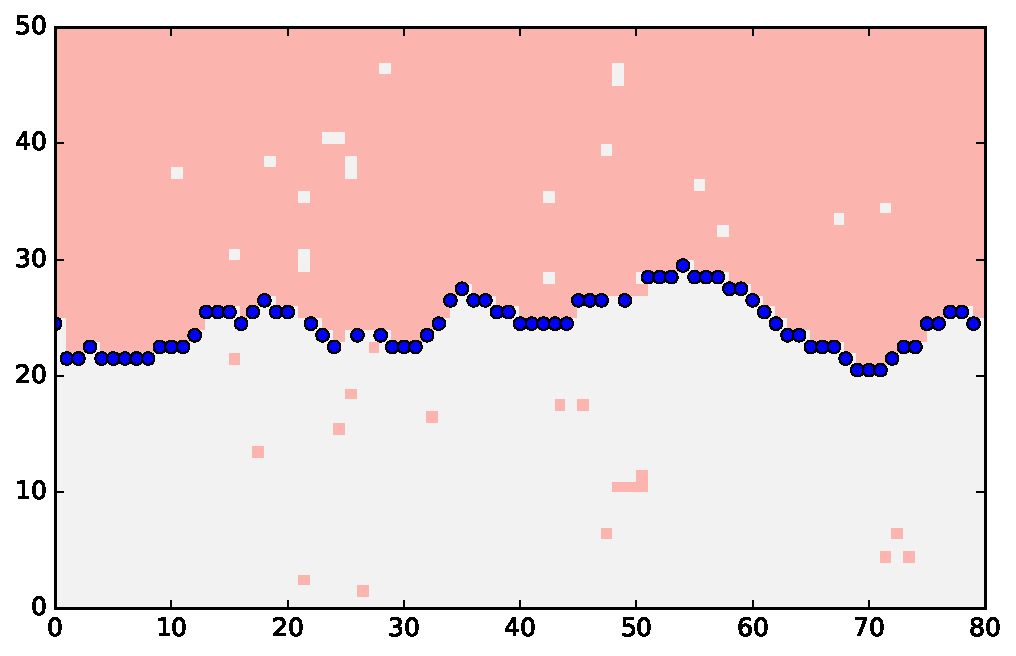
\includegraphics[width=\linewidth]{isingtosos/snap07.pdf}
	\end{minipage}%
	\begin{minipage}[t]{0.5\linewidth}
		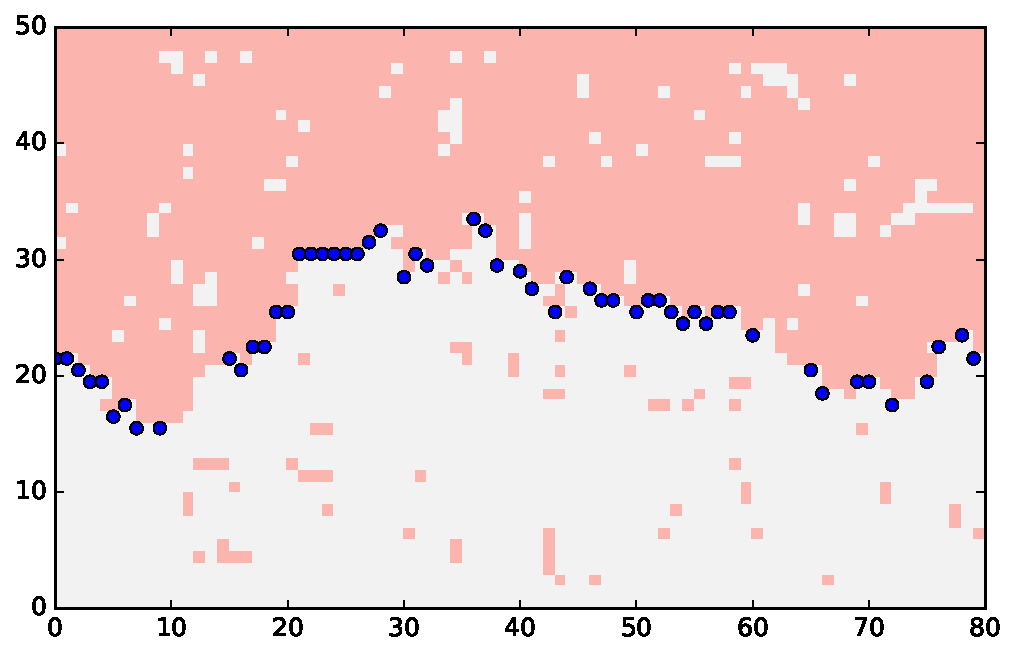
\includegraphics[width=\linewidth]{isingtosos/snap09.pdf}
	\end{minipage}
	\caption{Photo d'un modèle d'Ising à deux températures différentes($T=0.7 T_C$ et $T=0.95 T_C$ ) avec des conditions périodiques aux bords en X et fixés en Y qui forcent la présence d'une interface entre les phases $+$ (rose) et $-$ (blanc) du système. Plus la température est élevée et plus l'interface fluctue, jusqu'à cesser d'exister pour $T \greater T_C$. }
	\label{amas-fixe}
\end{figure}  
  
  	Le modèle d'Ising \footnote{Pour le lecteur curieux quant à l'histoire du modèle, se référer à \cite{niss_history_2005} et à \cite{niss_history_2009}.} est un modèle de particules sur réseau où l'interaction entre les particules du système se fait uniquement entre les plus proches voisins. Chaque particule au site $i$ possède deux états différents que l'on note $\sigma_i = \pm 1$, analogues aux spins en mécanique quantique. L'Hamiltonien d'un tel modèle s'écrit alors
\begin{equation}
	\mH =  - \sum_{<i j >} J_{ij} \sigma_i \sigma_j + \frac{V(i)+V(j)}{2}
	\label{hamil-ising}
\end{equation}
où $< ij >$ dénotent deux premiers voisins, $J_{ij}$ l'énergie d'interaction entre deux sites et $V(i)$ un champ externe. On peut voir ce terme d'interaction comme la discrétisation du terme $(\nabla \phi(\mx,t))^2$ où l'on a enlevé les constantes d'énergies, et l'absence du potentiel $\phi^4$ puisqu'il est toujours égal à $m^2+\frac{\lambda}{4!}$ ici. 

En faisant la transformation\cite{goldenfeld_lectures_2018} $n_i =  \frac{\sigma_i +1}{2}$ afin que $n_i(\sigma_i = 1) = 1$ et $n_i(\sigma_i = -1) = 0$, on obtient l'Hamiltonien
\begin{equation}
	\mH =  - \sum_{\langle i j >}  J_{ij} \left( 4 n_i n_j -2 ( n_i+n_j) + 1 \right)+ \sum_{\langle i j >}  J_{ij} \frac{V(\sigma_i)+V(\sigma_j)}{2}  
\end{equation}
où le terme constant $\sum_{\langle i j >}  J_{ij}$ ne modifie la fonction de partition $\mZ$ que d'une constante. On définit alors 
\begin{equation}
	\mH_{LG} =  - 4 \sum_{\langle i j >}  J_{ij}  n_i n_j  + 2 \sum_{\langle i j >}  J_{ij}  (n_i+n_j) + \sum_{\langle i j >}  J_{ij} \frac{V(\sigma_i)+V(\sigma_j)}{2}  
\end{equation}
Le deuxième terme s'identifie à la présence d'un potentiel chimique pour les particules liquide-gaz. Une phase magnétique positive dans le modèle d'Ising s'apparente dès lors à un état de haute densité (un liquide), tandis qu'une phase négative est considérée comme une phase de basse densité, c'est-à-dire un gaz.
Ce modèle représente également un mélange binaire entre deux types de particules $A$ et $B$ comme par exemple un polymère dans un solvant, les particules identiques s'attirent tandis que les particules d'un type différent se repoussent. 

\begin{figure}
    \centering
    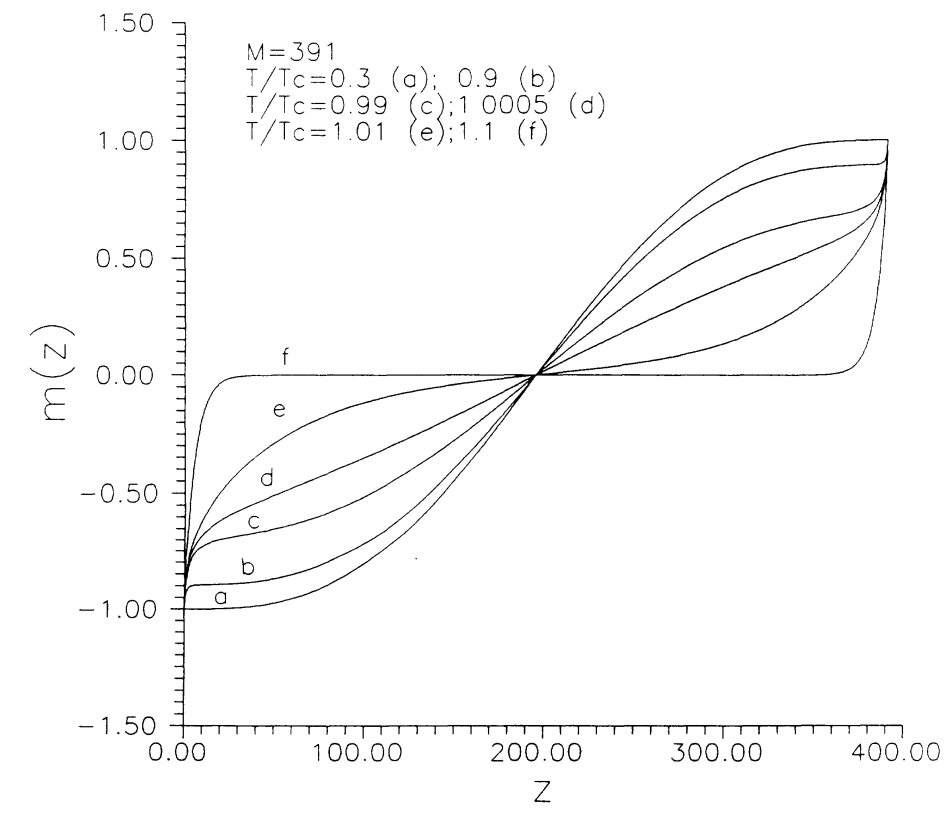
\includegraphics[width=0.5\linewidth]{isingtosos/stecki-profil.png}
    \caption{Profil de magnétisation $m(z)$ d'une interface en 2D pour différentes températures en unité de $T_C$ via la diagonalisation de la matrice de transfert du modèle d'Ising \cite{stecki_magnetization_1994}. Plus la température est faible  et plus elle est localisée.}
    \label{interface-ising}
\end{figure}

L'étude de l'interface entre les phases $+$ et $-$ nécessite la brisure de la symétrie de translation au sein du système. Cela peut se réaliser via des conditions aux bords non-périodiques dans une direction.
Dans ce cas par exemple, les spins de la rangée $0$ étant positifs et ceux de la rangée $L_Y$ négatifs, des clusters vont se former et créer une interface au milieu. 
Le profil de magnétisation d'une telle interface est donnée dans la figure \ref{interface-ising} \cite{stecki_magnetization_1994}, et sa tension superficielle est égale à \cite{abraham_transfer_1973,abraham_interface_1976,richards_numerical_1993} 
\begin{align}
    \sigma = 2 \beta J + \log(\tanh(\beta J))
\end{align}

Il est également possible de favoriser une phase par rapport à l'autre grâce à un champ externe assymétrique favorisant l'une des deux phases au-dessus et l'autre en-dessous, comme le potentiel $V(y) = - B |\frac{L_Y}{2}-y|$. Cette séparation modélise quant à elle l'effet d'un champ  sur un liquide binaire comme dans les expériences de forçage laser \cite{girot_conical_2019}, que nous étudierons plus en détail dans la Section \ref{sec_laser}.

%%%%%%%%%%%%%%%%%%%%%%%%%%%%%%%		
    \section{Hamiltonien}
%%%%%%%%%%%%%%%%%%%%%%%%%%%%%%%  
	
Quelle que soit la méthode utilisée, le système se simplifie dès lors que nous désirons étudier uniquement l'interface d'un système et non son ensemble, telles que les longueurs de corrélations dans le \textit{bulk}, l'aimantation moyenne, la chaleur spécifique ou la susceptilibté magnétique. À très basse température, les interfaces sont bien délimitées et il y a très peu de gouttes d'une phase dans l'autre. En considérant le système très peu mélangé, il est possible de définir la présence d'une phase par rapport à la hauteur $h_i$ de l'interface. Chaque site prend la valeur
\begin{align*}
	\sigma_{i,j} = \sgn(h_i-j)
\end{align*}
où la fonction $\sgn(x)$ est égale à $+1$ si $x>=0$ et à $-1$ sinon. Cela revient à considérer que l'énergie d'interaction perpendiculaire est prohibitive par rapport aux liaisons parallèles à l'interface $J_\perp \gg J_\parallel$. 

\begin{figure}
	\centering
	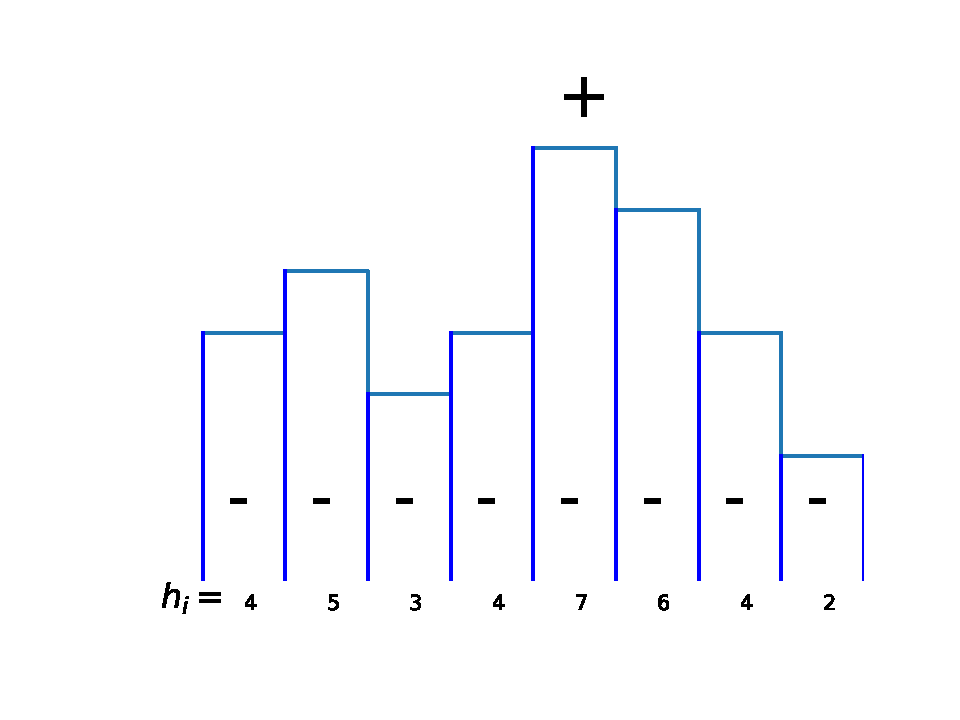
\includegraphics[scale=1]{isingtosos/sos-indiscernable.pdf}
	\caption{Une configuration possible de modèle SOS. Dans la i-ème colonne le bord horizontal de l'interface passe à la hauteur $h_i$. Toutes les particules au-dessus de l'interface sont des spins positifs et négatifs en dessous. La représentation classique du modèle SOS diffère de ce schéma par l'hypothèse que les particules sont discernables (cf figure \ref{figure-pop}).}
    \label{figure-sos}
\end{figure}


En utilisant les identités $2 \min(a,b) = |a+b| - |a-b|$ et $ 2\max(a,b)= |a+b| + |a-b|$, on a
\begin{align*}
    \sum_{j=0}^L \sgn(h-j)\sgn(h'-j) = L - 2 |h-h'|
\end{align*}
Ainsi, pour un système de longueur $L_X$ et de largeur $L_Y$ l'hamiltonien du modèle d'Ising \ref{hamil-ising} en l'absence de potentiel et en évitant de recompter les liens deux fois, se réécrit comme 
\begin{align}
    \mH = 2 J L_X (1-L_Y) +2 J \sum_i |h_i-h_{i+1}|
    \label{energie-sos-ising}
\end{align}
On peut également calculer directement l'énergie d'un tel système depuis une configuration SOS. Il existe $ L_Y$ liens verticaux par colonne, dont tous sauf un ont une énergie de $-J$, et le lien passant à travers l'interface ayant une énergie de $+J$. L'énergie totale des liens verticaux est donc de $E_y = - J L_X ( L_Y-2)$. De même pour les liens horizontaux, il existe $L_X \times L_Y$ liens au total, dont $\sum_i |h_i-h_{i+1}|$ liens d'énergie $+J$, ce qui nous donne une énergie d'interaction horizontale de $E_x = - J L_X L_Y + 2 \sum_i |h_i-h_{i+1}|$. La somme des deux énergies redonne \ref{energie-sos-ising}.

Le terme $|h_i-h_{i+1}|$ représente la surface de contact horizontale entre les deux phases qui dépend directement de la hauteur, tandis que le terme constant représente la surface de contact verticale.
En retirant la partie constante de l'énergie et simplifiant $2 J = J$ et en retirant l'énergie de volume qui est constante, nous obtenons l'hamiltonien du \textbf{modèle Solid-On-Solid} (SOS)
\begin{align}
    \mH = J \sum_{i=0}^{L_Y} |h_i-h_{i+1}|^k
    \label{hamil-sos}
\end{align}
L'exposant $k$ désigne ici tous les types de modèles SOS que l'on peut trouver avec des interactions différentes entres les sites. Par exemple, dans le cas d'un hamiltonien gaussien où  $k=2$, on peut démontrer qu'il existe une relation entre le modèle SOS et le modèle $XY$ \cite{knops_exact_1977}. Par la suite nous prendrons $k=1$ puisque c'est l'exposant qui découle directement de l'approximation du modèle d'Ising.

La dimensionalité du système a été réduite en ne prenant en compte que la hauteur $h_i$ au site $i$ à la place de la position de toutes les particules. L'approximation du modèle SOS implique que les configurations sont analogues à celles d'un mouvement brownien partiellement dirigé auto-évitant. Cette analogie a permis de diagonaliser complètement la fonction de partition dans le cas où il existe un champ magnétique et un potentiel épinglant l'interface (nous y reviendrons au paragraphe \ref{par-stab}) \cite{owczarek_exact_1993} et d'étudier les statistiques des déviations extrêmes de l'interface \cite{majumdar_airy_2005,schehr_universal_2006}.

En rajoutant la condition supplémentaire que $|h_i - h_{i+1} \leq 1$, on obtient que le \textbf{modèle Solid-On-Solid Restreint} (RSOS) \cite{privman_transfer-matrix_1989}. Ce modèle est une approximation du modèle SOS à très basse température.  Das ces conditions, l'interface est très lisse puisque l'on suppose que  \cite{kim_conserved_1994,vaysburd_critical_1995}. Dans la figure \ref{comparaison-modeles}, l'énergie du modèle d'Ising, du SOS et du RSOS sont reliées par l'équation \ref{energie-sos-ising}, et l'on voit que les approximations correspondent pour $T_{SOS} \less T_{C,Ising}$ et $T_{RSOS} \less T_{C,Ising}$. 

Par la suite, puisque nous désironts étudier le modèle SOS et non le comparer avec le modèle d'Ising, nous prendrons, sauf cas contraire explicité, $\beta = \beta_C \simeq 0.44$ et $J=1$. 

%%%%%%%%%%%%%%%%%%%%%%%%%%%%%%%%%%%%%%%
  \section{Matrice de Transfert}
%%%%%%%%%%%%%%%%%%%%%%%%%%%%%%%%%%%%%%%

	De manière plus générale, l'Hamiltonien d'un système avec des interactions entre les particules peut se réécrire comme $\mH = \sum_{\langle ij >} H(i,j)$ avec
\begin{align*}
  H(h_i,h_{i+1}) = f(h_i,h_{i+1}) + V(h_i,h_{i+1}) 
\end{align*}
où $f(h_i,h_j)$ est l'énergie d'interaction entre plus proches voisins et $V(h_i,h_j)=\frac{V(h_i)+V(h_j)}{2}$ le potentiel symmétrisé.
La fonction de partition de notre système s'écrit alors 

\begin{align*}
 Z = \sum_{h_1=0}^\infty \sum_{h_2=0}^\infty ... \sum_{h_L=0}^\infty e^{- \beta \sum_{i} H(h_i,h_{i+1})}  
   = \sum_{h_1 h_2 ... h_L} \prod_{i} e^{-\beta H(h_i,h_{i+1})} 
\end{align*}

La matrice 
\begin{align}
    T(h_i,h_j) = e^{-\beta H(h_i,h_j)}
    \label{matric-transfert}
\end{align}
est appelée matrice de transfert. Puisque le système est périodique (c'est-à-dire que $h_{L+1} = h_1$),  la matrice est périodique également, c'est-à-dire que $T(h_L,h_{L+1}) = T(h_L,h_1)$ \cite{pearce_exact_1989}. Elle est également symétrique, ce qui implique qu'elle est diagonalisable dans la base des vecteurs propres $|\lambda >$ de valeur propre $\lambda$. On dénote par $\lambda_0$ la plus grande valeur propre de $T$, par $\lambda_1$ la deuxième plus grande valeur propre et ainsi de suite.
Ainsi on peut diagonaliser la fonction de partition par la trace de la matrice de transfert \cite{abraham_transfer_1973}
\begin{align}
  Z = \sum_{h_1 h_2 ... h_L} \prod_{i} T(h_i,h_{i+i}) = Tr T^L  = \sum_\lambda \langle\lambda | T^L | \lambda> = \sum_\lambda \lambda^L
  \label{partition-trace-lambda}
\end{align}


\begin{figure}
    \begin{align}
    T = \begin{bmatrix} 
            \ddots & \vdots & \reflectbox{$\ddots$} \\ 
            e^{-\beta H(-1,-1)} &  e^{-\beta H(-1,0)} & e^{-\beta H(1,-1)} \\
            \dots & e^{-\beta H(0,0)} & \dots  \\
            e^{-\beta H(1,-1)} & e^{-\beta H(1,0)} & e^{-\beta H(1,1)}   \\ 
             \reflectbox{$\ddots$} & \vdots &\ddots  \\ 
        \end{bmatrix}
    \end{align}
    \caption{Matrice de transfert infinie et symmétrique \ref{matric-transfert}.}
\end{figure}

Dans la limite thermodynamique $L \to \infty$, seuls les plus grands vecteurs propres jouent un rôle. Afin de calculer les observables de notre système, il convient d'introduire les vecteurs de l'espace de Hilbert de ${|\lambda>}$ qui vont de $|h = -\infty>$ à $|h = +\infty>$.
En introduisant également la matrice des hauteurs $\tilde{M} |h> = h |h> i$, on trouve
\begin{itemize}
	\item L'énergie libre par site :  
	\begin{align}
		F =  - \frac{1}{L \beta} \ln(Z) \simeq - \frac{1}{\beta } \ln( \lambda_0)
		\label{energie-libre-site}
	\end{align}
	\item La densité de probabilité qu'un site se trouve à la hauteur $h$ :
	\begin{align}
		p(h) = \frac{1}{Z} \sum_\lambda \lambda^L \langle\lambda | h >^2 \simeq \langle \lambda_0 | h >^2
	\end{align}
	\item La magnétisation moyenne :
	\begin{align}
		M = \langle h > = \frac{1}{Z} \sum_\lambda \lambda^L \langle \lambda | \tilde{M} | \lambda \rangle \simeq \langle \lambda_0 | \tilde{M} | \lambda_0 > 
		\label{tm-magnetisation}
	\end{align}
	\item La variance des hauteurs :
	\begin{align}
		\sigma = \langle (h - \langle h >)^2 > = \frac{1}{Z} \sum_\lambda \lambda^L \langle \lambda | \tilde{M}^2 | \lambda \rangle - \langle \lambda | \tilde{M}| \lambda \rangle^2  \simeq  \langle \lambda_0 | \tilde{M}^2 | \lambda_0 >
	\end{align}
	\item La fonction de corrélation :
	\begin{align}
	    C(r) &= \langle h_i h_{i+r} \rangle - M^2 = \frac{1}{Z} \sum_{\lambda \neq \lambda_0} \langle \lambda_0 | M | \lambda \rangle \langle \lambda | M | \lambda_0 \rangle \left( \frac{\lambda}{\lambda_0} \right)^r  
	    \nn
	    &\simeq \langle \lambda_0 | M | \lambda_1 \rangle \langle \lambda_1 | M | \lambda_0 \rangle \left( \frac{\lambda_1}{\lambda_0} \right)^r
	\end{align}
	\item La longueur de corrélation :
	\begin{align}
	    \xi = - \frac{1}{\ln(\frac{\lambda_1}{\lambda_0})}
	    \label{longueur-correl-thermo}
	\end{align}
\end{itemize}

%%%%%%%%%%%%%%%%%%%%%%%%%%%%%%%%%%%%%
	\section{Stabilité de l'interface}
	\label{par-stab}
%%%%%%%%%%%%%%%%%%%%%%%%%%%%%%%%%%%%%

	Soit $\psi_\lambda(h)= <h|\lambda>$ la projection du vecteur propre associé à la valeur propre $\lambda$ de la matrice de transfert sur la base des hauteurs $|h>$ dans un système infini de part et d'autre de l'interface. En absence de potentiel\cite{guyer_sine-gordon_1979,chui_pinning_1981}, l'équation du vecteur propre donne
\begin{align}
	\sum_{h=-\infty}^\infty T(h,h') \psi_\lambda(h) = \lambda \psi_\lambda(h')
\end{align}
En introduisant l'ansatz $\psi_\lambda(h) = \alpha_{\lambda}^h$ et en séparant de la somme les termes pour $h$ négatifs et positifs, on trouve aisément que 
\begin{align}
	\lambda = \frac{\sinh(\beta J)}{\cosh(\beta J)-(\alpha_{\lambda}+\alpha_{\lambda}^{-1})} 
\end{align}
Dans la limite thermodynamique, la probabilité de présence de l'interface à la hauteur $h$ est $p(h) = <\lambda_0|h>^2 = |\psi_0(h)|^2$. Le système ne possédant aucune brisure de symétrie particulière, la probabilité $p(h)$ est finie pour tout $h$ avec $p(h)=p(-h)$. Dès lors, l'ansatz supposé $\psi_\lambda(h) = \alpha_{\lambda}^h$ implique que $\alpha_{\lambda}$ soit de la forme $e^{ik}$ où $k$ est la longueur d'onde associée à la valeur propre $\lambda$. On obtient que 
\begin{align}
	\psi_k(h) =& e^{ikh} \\
	\lambda =& \frac{\sinh(\beta J)}{\cosh(\beta J) - \cos(k)}
	\label{lambda-sos}
\end{align}

\begin{figure}
	\begin{minipage}[t]{0.5\linewidth}
		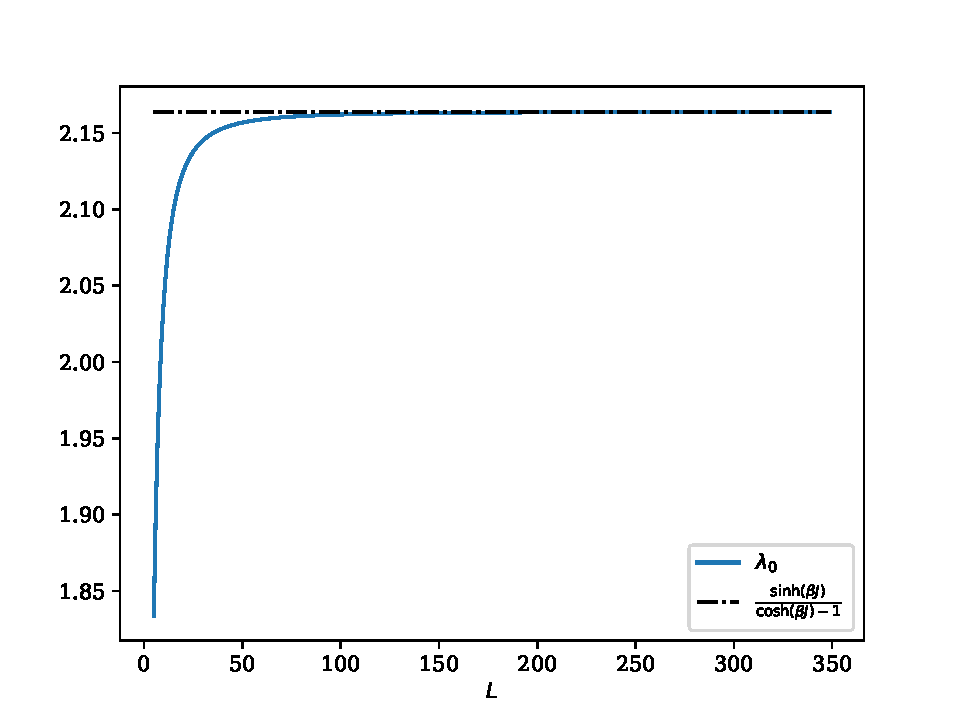
\includegraphics[width=\linewidth]{isingtosos/freeene-lambda0-libre.pdf}
	\end{minipage}%Cyclin
	\begin{minipage}[t]{0.5\linewidth}
		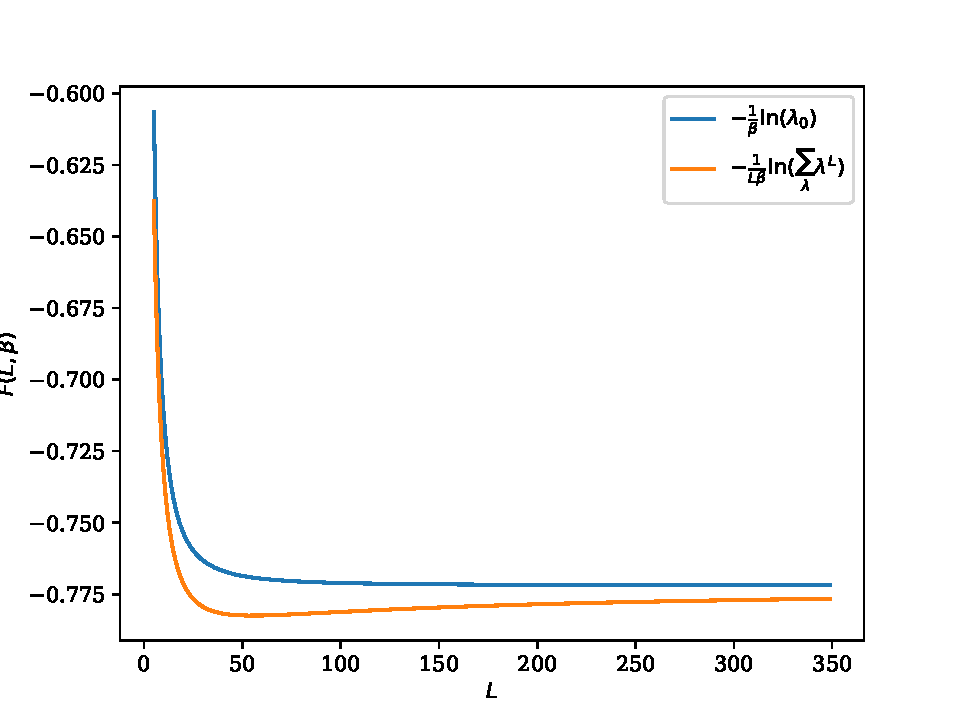
\includegraphics[width=\linewidth]{isingtosos/freeene-thermo-libre.pdf}
	\end{minipage}
	\caption{Plus grande valeur propre d'une interface libre en fonction de la taille $L$ du système  ayant pour limite \ref{lambda-sos} avec $k=0$ pour $\beta = 1$ (gauche)  ; énergie libre par site calculée via l'approximation de la limite thermodynamique \ref{energie-libre-site} comparé à la vraie fonction de partition \ref{partition-trace-lambda} en fonction de la taille $L$ du système pour $\beta = 1$ (droite).}
	\vspace{-0.5cm}
\end{figure}  

%Dans le cas plus général où la matrice de transfert s'écrit de la forme $T(h,h') = f(|h-h'|)$, on trouve 
%\begin{align}
%	\lambda = \sum_{h=0}^\infty f(h)(\alpha_{\lambda}^h+\alpha_{\lambda}^{-h}) - f(0)
%\end{align}

L'existence d'une solution de ce genre indique que l'interface n'est pas localisée dans le cas d'un système infini (ou semi-infini) en absence de tout potentiel, ce qui conduit à de nombreux problèmes numériques. 

Il est à noter qu'à $\beta=0$, c'est-à-dire pour une température infinie, tous les termes de la matrice de transfert sont égaux à $1$, menant à des vecteurs propres nuls. Dans cette limite, l'interface n'existe plus, le modèle SOS n'est donc pas valable. De même, pour une température nulle $\beta=\infty$, la matrice de transfert devient la matrice identité. Les valeurs propres deviennent toutes égales à $1$ et les vecteurs propres sont $\psi_i(h) = \delta_{h,i}$ où ici $i$ est l'indice de la i-ème valeur propre $\lambda_i = 1$. La probabilité de trouver l'interface à la hauteur $h$ devient $p(h) = \frac{1}{Z}\sum_{i} <\lambda_i | h >^2 = 1$. La température nulle a pour effet de geler l'interface sur une seule hauteur, mais toutes les hauteurs sont équiprobables. Bien que les micro-états soient extrêmement différents pour une température finie, les propriétés macroscopiques sont identiques à cause du même poids statistique associé à chaque état.


Une manière simple de localiser l'interface est de rajouter un potentiel $V(h) = -B \delta_{h,0}$ \cite{chui_pinning_1999,chalker_pinning_1981,chalker_pinning_1982}, qui augmente la probabilité de présence de l'interface à $h=0$. La recherche d'un état localisé nous donne un ansatz de la forme 
\begin{align}
	\psi_\lambda(h) = \begin{cases} |\alpha|^h & \text{si } h \neq 0 \\ \psi_{\lambda,0} & \text{sinon} \end{cases} 
\end{align}
L'équation du vecteur propre devient
\begin{align}
	\sum_{h=-\infty}^\infty e^{\beta |h-h'|- \beta B \delta_{h,0}} \psi_\lambda(h) = \lambda \psi_\lambda(h')
\end{align}
En notant $T(h,h') = R^{|h-h'|}$ pour $h \neq h' \neq 0$,  on obtient la même équation à un signe près dans l'exposant que l'on soit à $h'>0$ ou $h'>0$
\begin{align}
	\left( \frac{R}{\alpha} \right)^{\pm h'} \left[ \psi_{\lambda,0} + \frac{R \alpha}{1 - R \alpha} + \frac{\alpha}{R - \alpha} \right] + \left[ \frac{1}{1-R \alpha} - \frac{R}{R-\alpha} \right] = \lambda
\end{align}
Puisque cette équation est vraie pour tout $h'$, le premier terme doit être nul, ce qui nous donne
\begin{align}
	\psi_{\lambda,0} &= - \frac{\alpha}{R-\alpha}-\frac{R \alpha}{1-R \alpha} \\
	\lambda &= \frac{1}{1-R \alpha} - \frac{R}{R-\alpha}
\end{align}
L'équation du vecteur propre à $h'=0$ nous donne par ailleurs 
\begin{align}
	\psi_{\lambda,0} + 2 \frac{R \alpha}{1-R \alpha} = \lambda \psi_{\lambda,0} e^{-\beta B}
\end{align}
L'existence d'une solution cohérente $\alpha \less 1$ autorise la présence d'une interface localisée grâce à l'épinglage \cite{burkhardt_localisation-delocalisation_1981,kroll_solid--solid_1981,kroll_pinning_1982,kroll_interface_1983}.

D'autres méthodes existent pour confiner l'interface. Le cisaillement d'une interface diminue sa largeur et permet de la localiser dans l'espace. On peut également proposer deux potentiels chimiques différents pour chaque phase à une hauteur de l'interface prédéfinie, comme le ferait un laser dans un liquie binaire dont chaque phase  a un incident de réfraction différent \cite{casner_laser-induced_2003,delville_laser_2009} (voir chapitre \ref{sec_laser}). Dans un système infini, une autre possibilité est de définir un champ magnétique symétrique rendant plus difficile la présence de l'interface loin de $0$. Nous utiliserons ici un potentiel du style
\begin{align}
		  V(h) = B |h|
\end{align}

Il est facile de se convaincre que loin de $h=0$ l,e coût énergétique est si grand que la probabilité que l'interface s'y trouve soit petite, impliquant que l'interface est localisée. La position moyenne de l'interface se situe au minimum du potentiel qui est dans ce cas $0$. 

%%%%%%%%%%%%%%%%%%%%%%%%%%%%%%%%%%%%%%%%%%%
	\section{Équivalence des ensembles}
%%%%%%%%%%%%%%%%%%%%%%%%%%%%%%%%%%%%%%%%%%%

\begin{figure}[h]
	\centering
	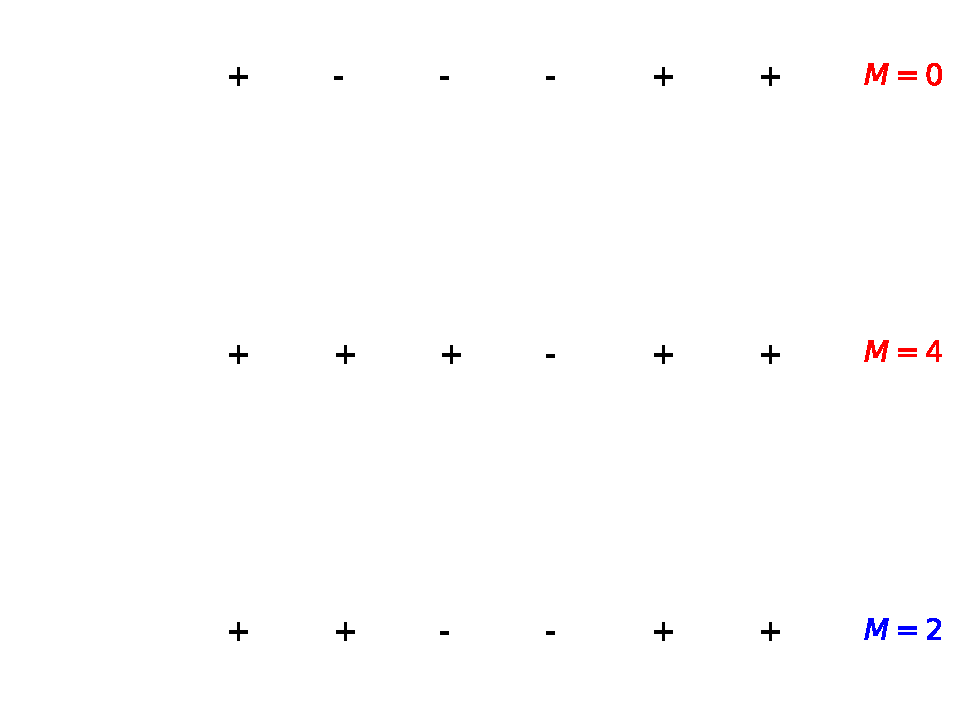
\includegraphics[scale=1]{isingtosos/figure-canonique.pdf}
	\caption{Dans un modèle d'Ising à 1D, afin d'avoir une magnétisation moyenne du système à $<M>=2$, tous les états sont acceptés tant qu'il y en a d'autres afin de respecter la moyenne. Dans l'ensemble canonique, on n'a plus $<M>=2$ mais $M=2$, interdisant les micro-états rouges.}
\end{figure}

Dans l'ensemble grand-canonique, le nombre de particules dans le système varie, dépendant du potentiel chimique vis-à-vis du réservoir dans lequel il est inséré, ce qui permet à l'interface de bouger librement. Lorsque l'on se place dans un système canonique, l'aire totale $A$ de l'interface est fixe, ce qui introduit une contrainte dans la fonction de partition
\begin{align}
	 Z(A) = \sum_{h_1 h_2 ... h_L} e^{- \beta \sum_{i} H(h_i,h_{i+1})}  \delta(\sum_i h_i = A)
	 \label{hamil-sos-cano}
\end{align}
La position moyenne de l'interface est maintenant imposée, ce qui interdit beaucoup de microétats, ce qui change  les propriétés thermodynamiques de la matrice de transfert comme la distribution des hauteurs de l'interface \cite{siegert_scaling_1993}, même si la moyenne reste la même. Dans la limite thermodynamique, si l'on prend dans l'ensemble canonique pour paramètre d'ordre la valeur moyenne du paramètre d'ordre dans l'ensemble grand canonique, on s'attend à ce que les observables du système se comportent de manière équivalente. 
Malheureusement, il est impossible de réécrire la contrainte dans le langage des matrices de transfert, empêchant ainsi de calculer analytiquement les différences entre les deux ensembles pour une taille donnée. Il est possible de construire la fonction de partition \textit{ab initio}, mais le grand nombre de sites et de hauteurs permises dans un système classique empêchent le calcul dans un temps CPU raisonnable. 

La fonction de partition \ref{hamil-sos-cano} est en relation vis-à-vis de l'ensemble grand-canonique grâce  au potentiel chimique $\mu$ par
\begin{align}
	 \Xi(\mu) = \sum_{A = -\infty}^\infty Z(A) e^{\beta \mu A}
\end{align}
avec pour nouvelle matrice de transfert
\begin{align}
    T(h_i,h_j) = e^{-\beta |h_i-h_j| + \beta \mu \frac{h_i+h_j}{2}}
    \label{tm-sos-grand-cano}
\end{align}

\begin{figure}
    \centering
	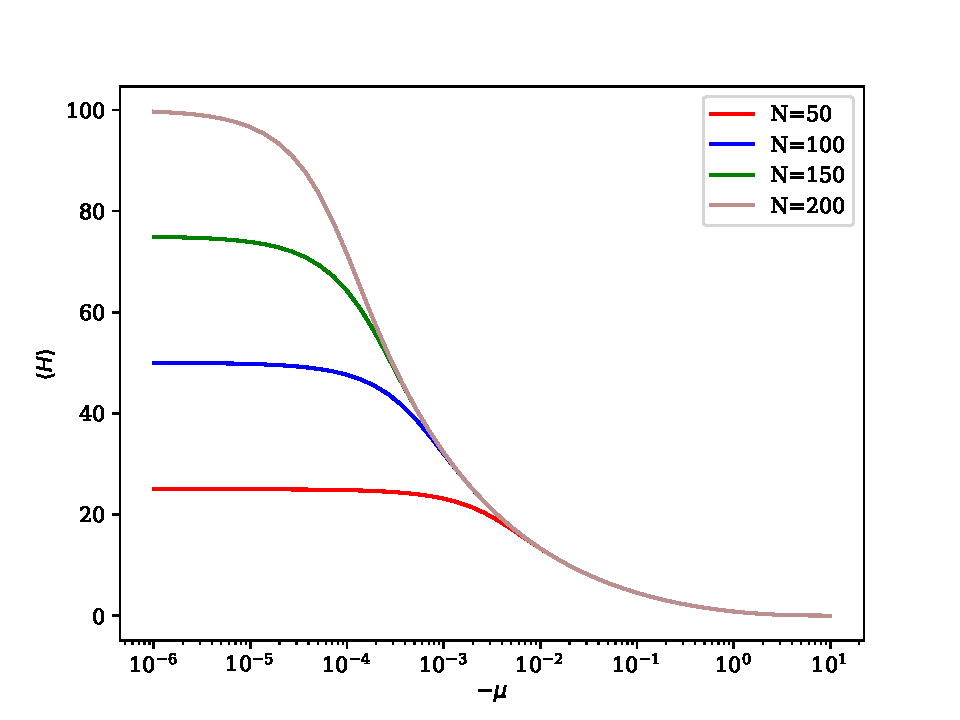
\includegraphics[width=0.5\linewidth]{isingtosos/hauteur-tm-sos.pdf}
	\caption{Position d'équilibre de l'interface \ref{tm-sos-grand-cano} en fonction de $- \mu$ via diagonalisation de la matrice de transfert \ref{tm-sos-grand-cano}. Lorsque le potentiel chimique est trop faible, l'interface est délocalisée et se retrouve à la position $\frac{N}{2}$. }
	\label{hauteur-mu}
\end{figure}

%%%%%%%%%%%%%%%%%%%%%%%%%%%%%
	\section{Modèle de particules : le modèle POP}
%%%%%%%%%%%%%%%%%%%%%%%%%%%%%

\begin{figure}[h]
	\centering
	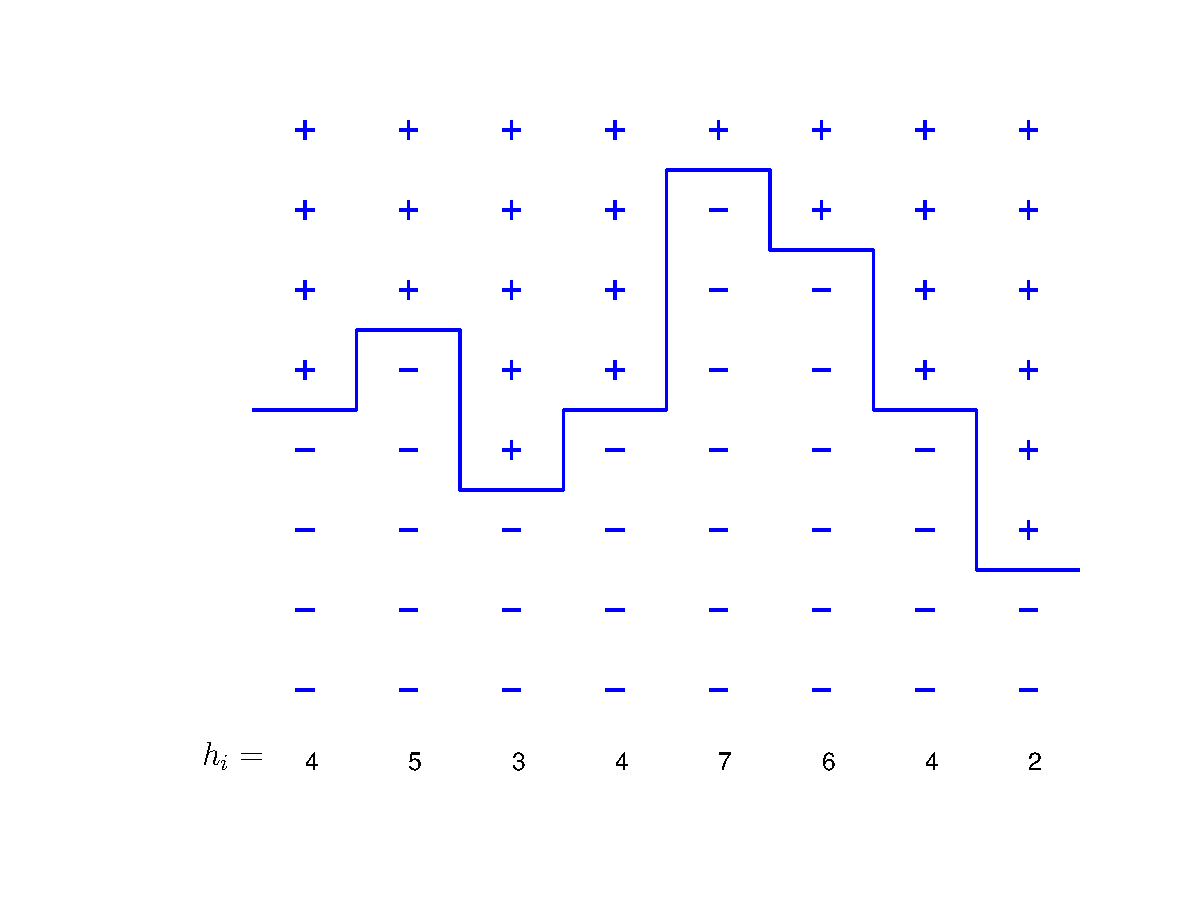
\includegraphics[width=0.7\linewidth]{isingtosos/figure-sos.pdf}
	\caption{Position d'équilibre de l'interface \ref{tm-magnetisation} en fonction de $\mu$ via diagonalisation de la matrice de transfert \ref{tm-sos-grand-cano}.}
	\label{figure-pop}
\end{figure}	
\begin{figure}
	\centering
	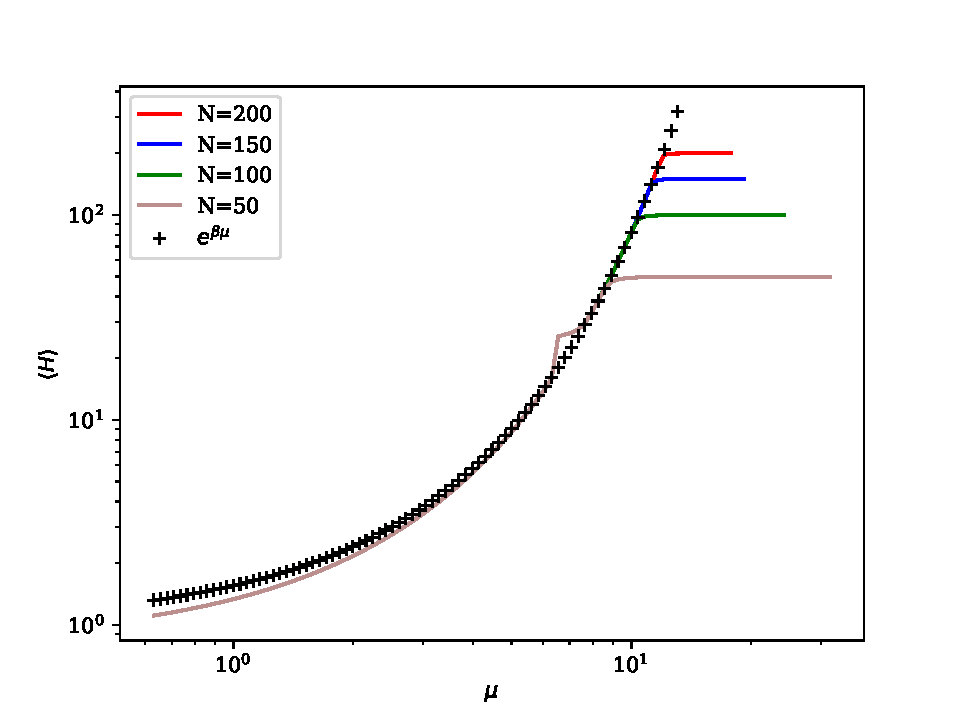
\includegraphics[width=0.5\linewidth]{isingtosos/hauteur-tm-pop.pdf}
	\caption{Position d'équilibre de l'interface \ref{tm-magnetisation} en fonction de $\mu$ via diagonalisation de la matrice de transfert \ref{hamil-pop}. La solution analytique \ref{position-hauteur-pop} (en pointillés) correspond lorsque le potentiel chimique n'est plus négligeable. La bosse à $\mu \simeq 7$ est due à un overflow dans le calcul de la matrice de transfert sous Python.}
	\label{figure-pop}
\end{figure}
	
Lorsque nous avons fait l'approximation SOS dans le modèle d'Ising, nous sommes passés d'un système où l'on prenait en compte toutes les interactions entre particules vers un modèle d'interface où seul comptent les particules au niveau de l'interface, perdant ainsi l'information sur le bulk. Chaque site $i$ est maintenant définit par la coordonnée de la hauteur de l'interface $h_i$, dont l'entropie est donnée par les permutations possibles des hauteurs.
Nous proposons ici un nouveau modèle, où nous n'avons pas perdu l'information sur la position des particules, que nous nommerons \textbf{le modèle Particles-Over-Particles} (POP). Soit $N = \sum_i h_i$ le nombre de spins $+$ dans le système, c'est-à-dire l'aire sous l'interface.
La grande fonction de partition devient
\begin{align}
    \Xi(\mu) = \sum_{{\bf h_i }} e^{- \beta J \sum_{i} |h_i-h_{i+1}| + \beta \mu \sum_i h_i  - \sum_i \ln(h_i !)} 
    \label{hamil-pop}
\end{align}
où le second terme provient du fait qu'il y a $N! / \Pi_i h_i! $ manières de choisir les configurations spécifiées par les $h_i$ parmi les $N = \sum_i h_i$ particules qui sont indiscernables entre elles. 
Le potentiel effectif contient le potentiel chimique ainsi que l'effet de l'entropie
\begin{align}
    V_e = \beta \mu \sum_i h_i - \sum_i \ln(h_i!)
\end{align}
Grâce à la formule de Stirling pour $h_i$ grand, et en considérant une configuration où l'interface est lisse $h_i = <h>$, on a
\begin{align}
    \frac{dV}{d<h>} = 0 \rightarrow <h> = e^{\beta \mu} + C
    \label{position-hauteur-pop}
\end{align}
Dans la limite $\mu \to -\infty$, aucune particule ne peut se déposer dans le système, et donc $C=0$.



%%%%%%%%%%%%%%%%%%%%%%%%%%%%%%%
\section{Conclusion}
%%%%%%%%%%%%%%%%%%%%%%%%%%%%%%%

Bien que le modèle d'Ising soit extrêmement étudié de par sa richesse au niveau de la transition de phase, l'étude des interfaces peut se contenter d'une approximation à basse température où il n'existe pas d'évaporation, bulles ou digitations de la phase $+$ au sein de la phase $-$ et vice-versa. Le modèle Solid-On-Solid suffit à étudier une grande variété de phénomènes ayant lieu à l'interface d'Hamiltonien \ref{hamil-sos}. 
La basse dimensionalité de ce système permet d'utiliser le formalisme des matrices de transfert. 
Nous avons démontré que l'interface était libre de fluctuer où elle le désirait sauf en présent d'un champ de confinement qui permet d'étudier ses fluctuations autour d'un point central.
La prise en compte des permutations possibles des particules ajoute un terme d'entropie à la fonction de partition. Ce nouveau modèle, baptisé POP, possède de nombreuses propriétés nouvelles qui le rapprochent du modèle d'Ising.

\begin{figure}
    \centering
    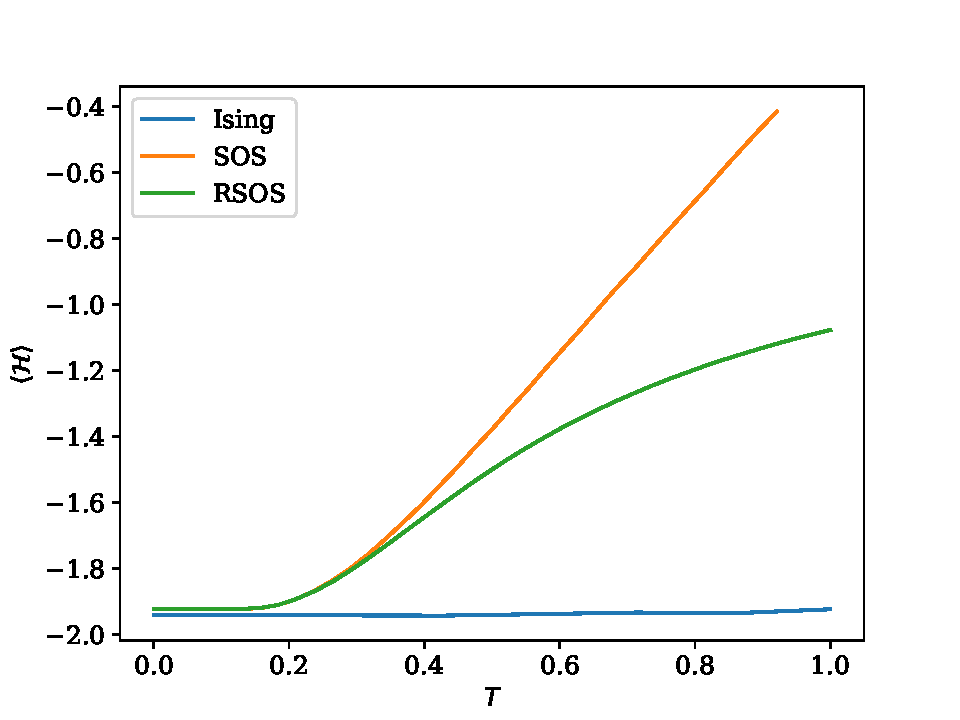
\includegraphics[width=0.5\textwidth]{isingtosos/comparaison-modeles.pdf}
    \caption{Énergie par site entre les modèles d'Ising (\ref{hamil-ising}) (avec conditions fixes en $y$), SOS et RSOS (\ref{hamil-sos}) et POP (\ref{hamil-pop}) en fonction de la température via des simulations de Monte Carlo pour $L_X=64$, $L_Y=51$ et $J=1$ avec des conditions périodiques en $x$. La configuration intiale est la configuration à $T=0$ d'une interface parfaitement lisse. {\color{red} Besoin refaire Ising avec MCIA.} }
    \label{comparaison-modeles}
\end{figure}